\documentclass{beamer}

\title{Modelos Generativos Profundos}
\subtitle{Clase 1: Introducción}
\author{Fernando Fêtis Riquelme}
\institute{
    Facultad de Ciencias Físicas y Matemáticas\\
    Universidad de Chile
}
\date{Otoño, 2025}
\titlegraphic{\hfill
\includegraphics[height=1.2cm]{fcfm}}

\usetheme{metropolis}
\setbeamercovered{transparent}

\begin{document}

\begin{frame}
    \titlepage
\end{frame}

\begin{frame}{Clase de hoy}
    \tableofcontents
\end{frame}

\section{Introducción a los modelos generativos modernos}

\begin{frame}{Qué son los modelos generativos y cómo funcionan}
    \begin{itemize}
        \item<1> Qué es un modelo generativo.
        \item<2> Aprendizaje supervisado vs. no supervisado.
        \item<3> Criterios de aprendizaje.
        \item<4> Generación condicional.
    \end{itemize}
\end{frame}

\begin{frame}{Qué puede generar un modelo generativo}
    Se pueden realizar múltiples tareas usando modelos generativos.
    \begin{itemize}
        \item<2> Creación y modificación de imágenes.
        \item<3> Generación de sonido y video.
        \item<4> Simular juegos.
        \item<5> LLMs en robótica.
        \item<6> Predicción de estructuras moleculares.
        \item<7> Otros estudios científicos.
    \end{itemize}
\end{frame}

\begin{frame}{Perspectivas para estudiar modelos generativos}
    Los modelos generativos actuales pueden ser estudiados desde distintos ángulos
    \begin{itemize}
        \item<2> Perspectiva económica y social.
        \item<3> Perspectiva ética.
        \item<4> Interés filosófico.
        \item<5> Interés teórico.
    \end{itemize}
\end{frame}

\begin{frame}{Qué se estudiará en este curso}
    Se comenzará estudiando las \textbf{redes bayesianas}. Luego, se estudiarán los 6 principales paradigmas generativos.
    \begin{enumerate}
        \item<2> Modelos autorregresivos (ARMs).
        \item<3> Redes generativas adversarias (GANs).
        \item<4> Autoencoders variacionales (VAEs).
        \item<5> Modelos basados en energía (EBMs).
        \item<6> Modelos de difusión (DMs).
        \item<7> Flujos normalizantes (NFs).
    \end{enumerate}
\end{frame}

\begin{frame}{Qué no se estudiará en este curso}
    Los siguientes temas son importantes, pero solo serán mencionados en este curso.
    \begin{itemize}
        \item<2> Prompt engineering.
        \item<3> Temas de ML engineering.
        \item<4> Uso de frameworks de IA.
        \item<5> Métodos generativos \textit{antiguos}.
        \item<6> Enfoques híbridos.
        \item<7> Alignment.
    \end{itemize}
\end{frame}

\section{Requisitos y evaluaciones del curso}

\begin{frame}{Requisitos del curso}
    Si bien el curso es autocontenido, se asumen algunos conocimientos previos.
    \begin{itemize}
        \item<2,4> \textbf{Probabilidades:} distribuciones clásicas, variables independientes, probabilidad condicional, regla de Bayes, marginalización, verosimilitud, esperanza, etc.
        \item<3,4> \textbf{PyTorch:} creación de datasets, redes fully-connected, redes convolucionales, entrenamiento de modelos, etc.
    \end{itemize}
    \uncover<4>{Se realizará un repaso breve de estos temas en la siguiente clase.}
\end{frame}

\begin{frame}{Evaluaciones}
    Hay dos tipos de evaluación en el curso.
    \begin{itemize}
        \item<2,4> \textbf{Tareas (70\%):} una tarea por paradigma (6 en total).
        \item<3,4> \textbf{Proyecto final (30\%):} implementación minimal de un paper.
    \end{itemize}
    \uncover<4>{Ambos items deben ser aprobados por separado para aprobar el curso.}
\end{frame}

\begin{frame}{Evaluaciones}
    Algunas consideraciones.
    \begin{itemize}
        \item<2> Las tareas se hacen en pareja o de forma individual. El proyecto en grupos de 4 personas.
        \item<3> Se elimina la peor nota de las tareas.
        \item<4> Cada día de atraso en la entrega de una tarea implica el descuento de 1 punto.
        \item<5> Se pueden usar herramientas tipo ChatGPT, pero, para cada tarea, un grupo de personas presentará al azar su solución.
    \end{itemize}
\end{frame}

\section{Calendario y bibliografía}

\begin{frame}{Plan de clases (tentativo)}
    Los temas que se revisarán para cada paradigma generativo son los siguientes:
    \begin{table}[h]
        \centering
        \resizebox{\columnwidth}{!}{
            \begin{tabular}{|c|c|c|c|c|}
                \hline
                \textbf{Tema}         & \textbf{Clase 1} & \textbf{Clase 2}       & \textbf{Clase 3} & \textbf{Clase 4} \\ \hline
                \textbf{Introducción} & primera clase    & repaso previo          & redes bayesianas & ejemplos         \\ \hline
                \textbf{ARMs}         & formulación      & implementación GPT     & propiedades      & ejemplos         \\ \hline
                \textbf{GANs}         & implementación   & image-to-image         & propiedades      &                  \\ \hline
                \textbf{VAEs}         & formulación      & implementación         & VQ-VAE           &                  \\ \hline
                \textbf{EBMs}         & score matching   & denoising SM           & otras variantes  &                  \\ \hline
                \textbf{DMs}          & forma discreta   & generación condicional & ejemplos         & forma continua   \\ \hline
                \textbf{NFs}          & formulación      & implementación         & ejemplos         &                  \\ \hline
            \end{tabular}
        }
    \end{table}
    Las 3 semanas restantes serán dedicadas al proyecto final.
\end{frame}

\begin{frame}{Libros de referencia}
    Hay 3 libros que se recomiendan para el curso. El 1º sirve como introducción a cada tema, el 2º contiene la formalidad matemática, y el 3º contiene implementaciones en PyTorch.
    \vspace{0.3cm}
    \begin{center}
        \href{https://www.oreilly.com/library/view/generative-deep-learning/9781098134174/}{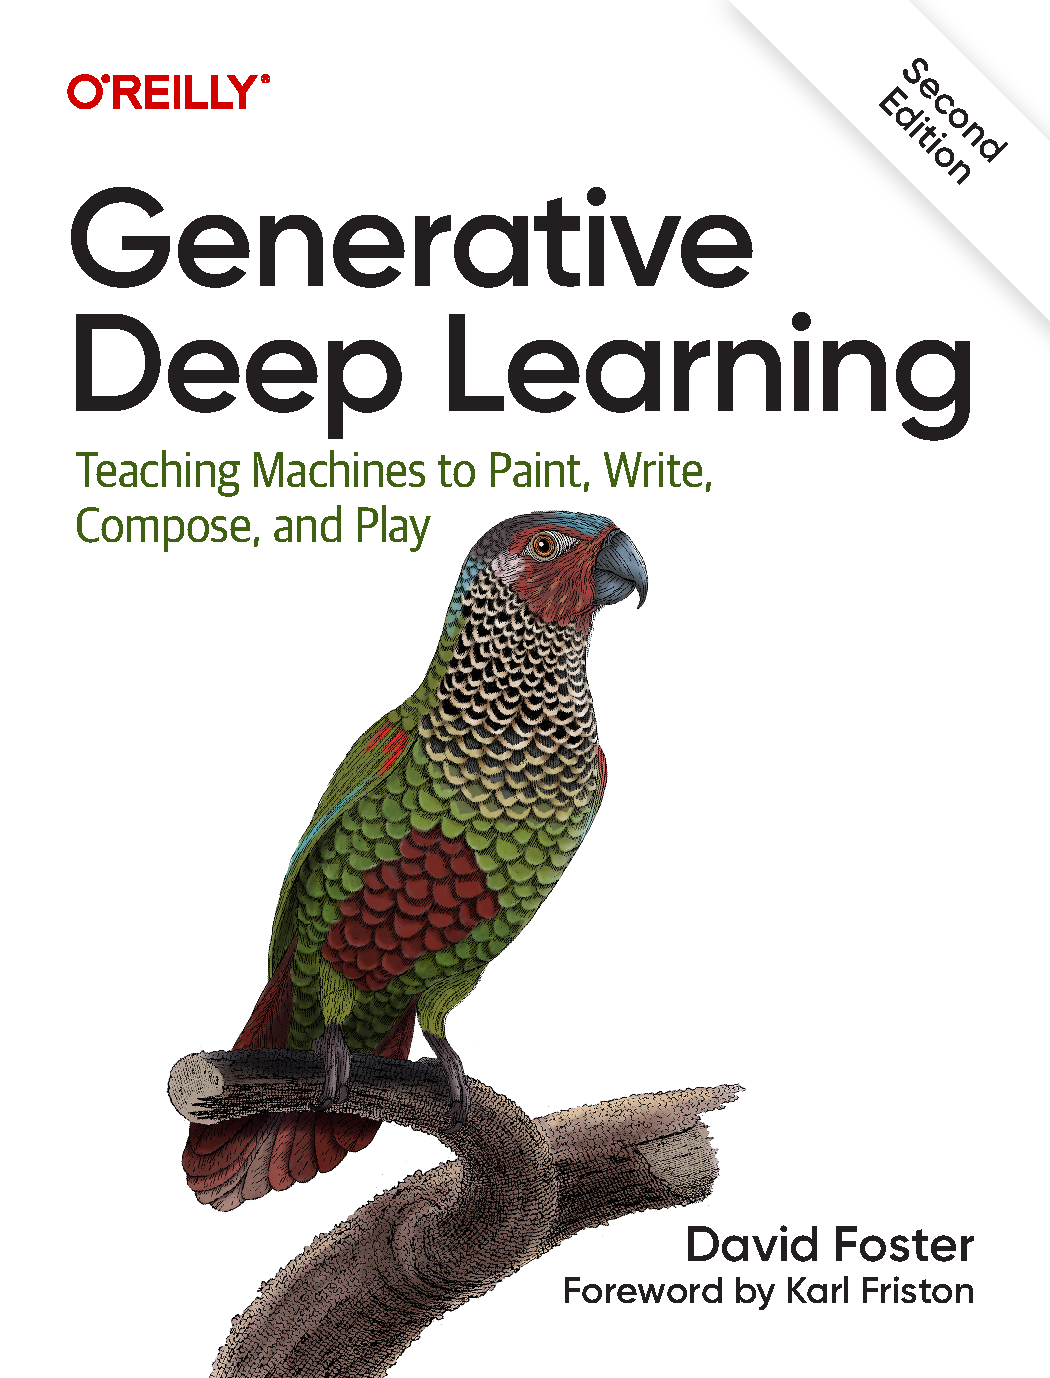
\includegraphics[width=0.3\textwidth]{foster.pdf}}
        \href{https://probml.github.io/pml-book/book2.html}{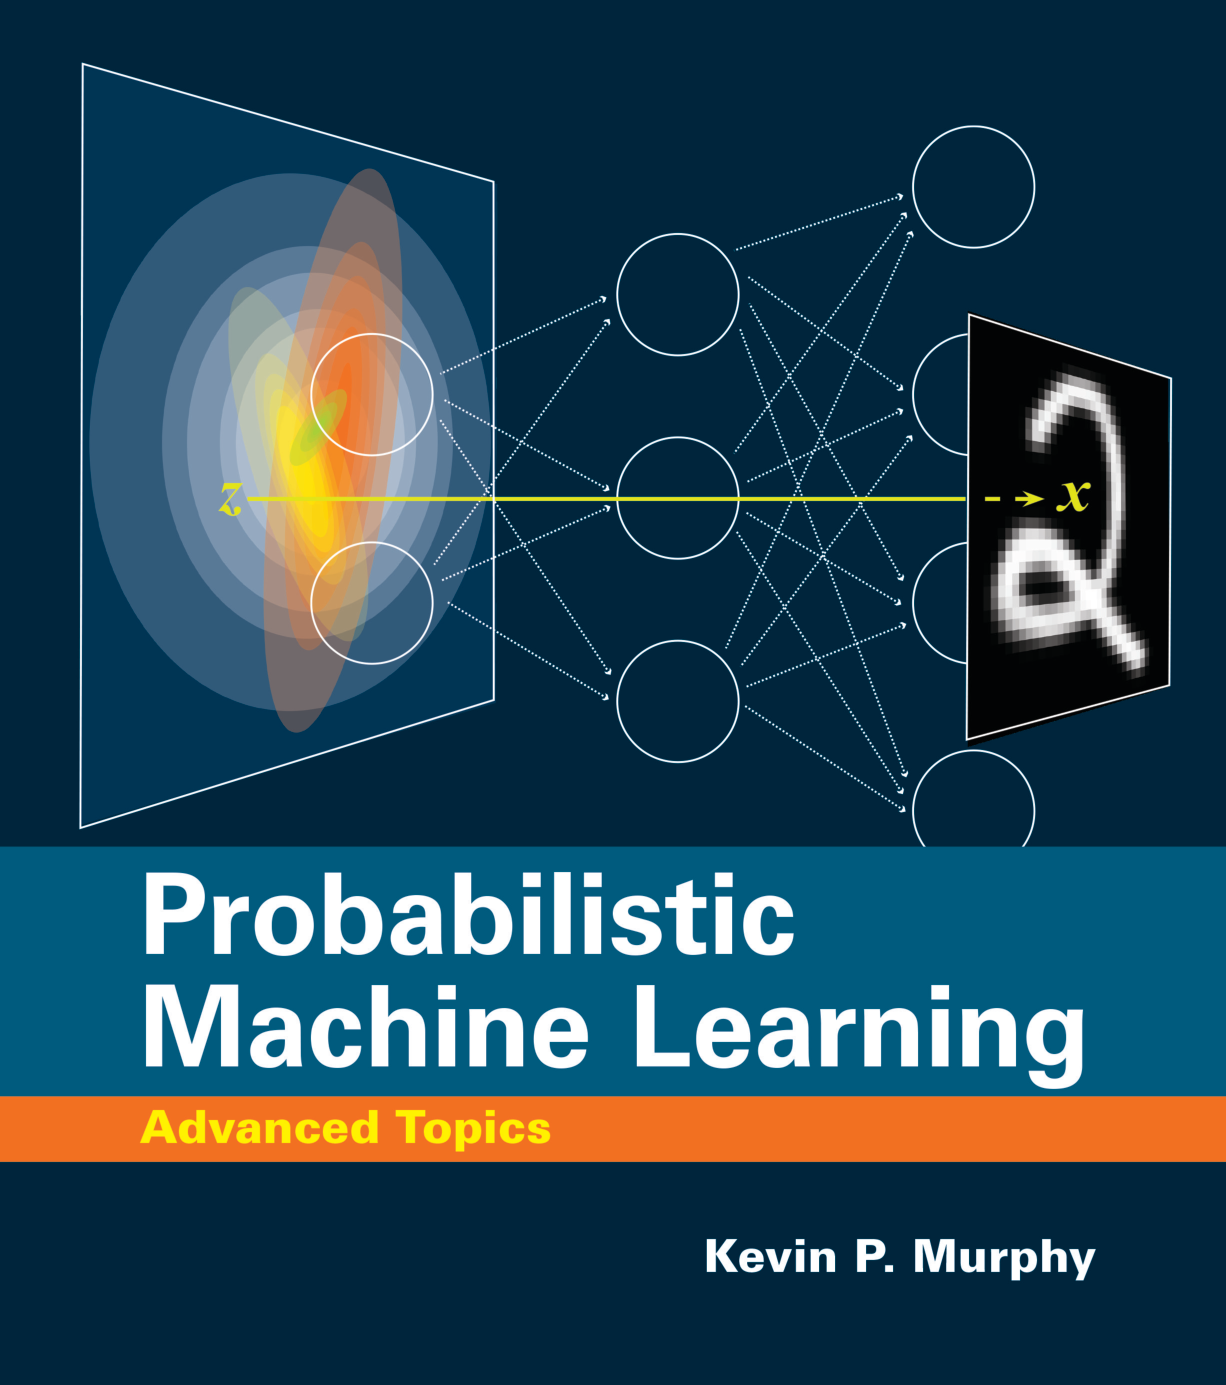
\includegraphics[width=0.3\textwidth]{murphy.pdf}}
        \href{https://link.springer.com/book/10.1007/978-3-031-64087-2}{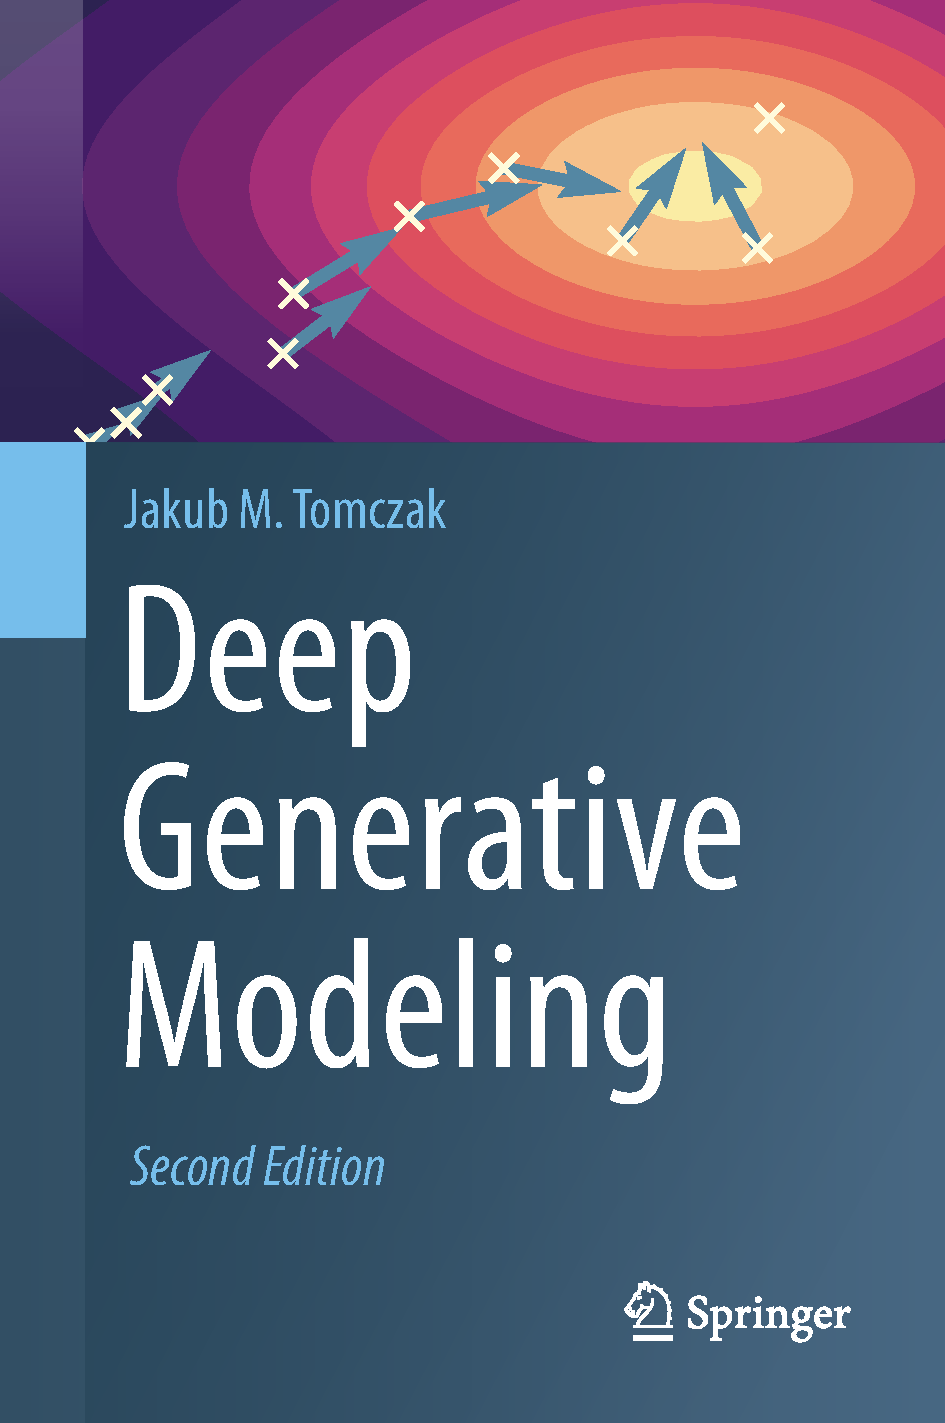
\includegraphics[width=0.3\textwidth]{tomczak.pdf}}
    \end{center}
\end{frame}

\begin{frame}{Próxima clase}
    En la próxima clase.
    \begin{itemize}
        \item<2> Se hará un repaso de conceptos de probabilidad y de PyTorch necesarios para el curso.
        \item<3> Se introducirán las redes bayesianas.
    \end{itemize}
\end{frame}

\begin{frame}
    \centering
    \Large{Modelos Generativos Profundos}\\
    \large{Clase 1: Introducción}
\end{frame}

\end{document}